\chapter{MUD CONDITIONING EQUIPMENT}


\textbf{Mud Pump:} Sucks mud from the mud pits and pumps it to the drilling apparatus.

\vspace{1em}

\noindent \textbf{Shale shaker:}Separates rock cuttings from the mud.

\vspace{1em}

\noindent \textbf{Mud pit:} In mud pits drilling mud is mixed and recycled. 

\vspace{1em}

\noindent \textbf{Reserve pit:} It collects rock cuttings separated from the mud.

\vspace{1em}

\noindent \textbf{Mud-mixing hopper:} In this new mud is mixed and then sent to the mud pits.

\vspace{1em}

\noindent \textbf{Desander and Desilter:} In desander sand particles are removed while in desilter small silt particles are removed.

\vspace{1em}

\noindent Figure 4.1 shows theimage of Mud Conditing Equipment.

\vspace{1em}

\begin{figure}[h]
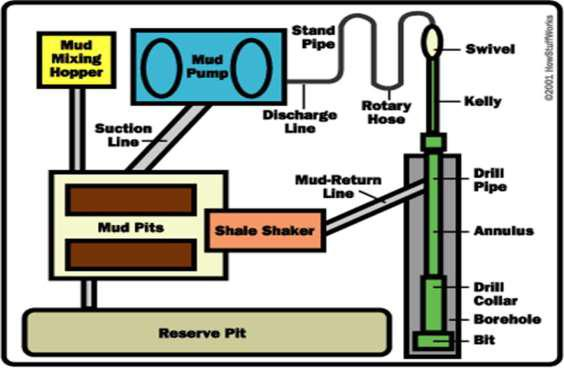
\includegraphics[scale=0.6]{images/Mudconditingequipment}
\centering 
\caption{A Picture of Mud Conditing Equipment}
\end{figure}



% Have to insert a figure at the end of this page.